\subsection{Fall Update 3}
Progress since last week:
\begin{itemize}
\item We have finished the requirements document after having our client review it.
\item We received our Raspberry Pi and touchscreen hardware.
\end{itemize}
Problems:
\begin{itemize}
\item No problems this week.
\end{itemize}
Plans for the coming week: 
\begin{itemize}
\item Begin working on the Pi starting with an operating system and then branching out to communication between the devices and touchscreen capabilities.
\end{itemize}
Blog Date: 10-29-15


\subsection{Fall Update 4}
Most of what we did this week involved trying to get a functioning proof of concept for our project, which turned out to be filled with more problems than anticipated. We began to investigate software packages and technologies that would help us meet the requirements outlined on our document. We will hopefully have a functional proof-of-concept by the next week.\\
Progress since last week:
\begin{itemize}
\item Tested the devices with various wireless networking methods, including ad-hoc and in access-point mode
\item Continued to develop our documents such as the technical requirements and elevator pitch
\end{itemize}
Problems:
\begin{itemize}
\item The ad-hoc system did not work as expected due to the USB WiFi adapters we were using, and we had to reevaluate​ our network implementation
\end{itemize}
Plans for the coming week: 
\begin{itemize}
\item Continue to develop a proof-of-concept, working with a new structure with the wireless components that will function to expectations.
\end{itemize}
Blog Date: 11-5-15

\subsection{Fall Update 5}
Progress since last week:
\begin{itemize}
\item We now have a working proof of concept where the Pi is able to wirelessly communicate to the ESPs and cause each of the connections on the relays to be activated individually.
\item Completed technology review and revision of requirements document.
\item Started on expo poster.
\end{itemize}
Problems:
\begin{itemize}
\item No real problems other than having to revise the requirements document to be more detailed and fine-grained.
\end{itemize}
Plans for the coming week: 
\begin{itemize}
\item Finish Poster
\item Revise elevator pitch
\item Demonstrate proof of concept
\item Possibly attach actual lights to the relay rather than just using the relay's LEDs to see which switches are enabled.
\end{itemize}
Blog Date: 11-13-15

\subsection{Fall Update 6}
Progress since last week:
\begin{itemize}
\item Our proof of concept is now portable, and booting the pi connects it to the ESP8266 module and cycles the lights on the relay.​ It has also been shown to the TA.
\item Finished expo poster
\item Re-wrote elevator pitch
\end{itemize}
Problems:
\begin{itemize}
\item No real problems this week
\end{itemize}
Plans for the coming week: 
\begin{itemize}
\item Continue to develop the proof of concept, possibly by adding actual lights to the relay instead of the LED's.
\item Present the elevator pitch​
\end{itemize}
Blog Date: 11-19-15

\subsection{Fall Update 7}
Progress since last week:
\begin{itemize}
\item We have connected actual lights to our relay and verified that they can be toggled on/off.
\item We have presented our elevator pitch.
\item We have begun learning how to use Flask for our website.
\end{itemize}
Problems:
\begin{itemize}
\item No real problems this week
\end{itemize}
Plans for the coming week: 
\begin{itemize}
\item Work on our design document​
\item Become more familiar with Flask and potentially start on the website
Use the Yocto build server to build the new system rather than using Raspbian.
\item Work on progress report
\end{itemize}
Blog Date: 11-28-15


\subsection{Fall Update 8}
Progress since last week:
\begin{itemize}
\item We retrieved our build server from Kevin and installed Linux. We also installed the Yocto build system and built core-image-minimal to verify that it works. 
\item We booted the Raspberry Pi with core-image-minimal to verify that the images would work
\item We investigated options for connections and user experiences, and decided on a wireless connection method for our system
\item We completed our design document and ran it by our TA. We also continued work on the progress report.
\end{itemize}
Problems:
\begin{itemize}
\item We had a bit of a confused discussion on the user experience complexity and the wireless communication methods we would use, as we did not know the expectations for ease-of-use. We contacted Victor and had our questions answered.
\end{itemize}
Plans for the coming week: 
\begin{itemize}
\item Work on our report
\item Over break, start to build the web framework with Flask. 
\end{itemize}
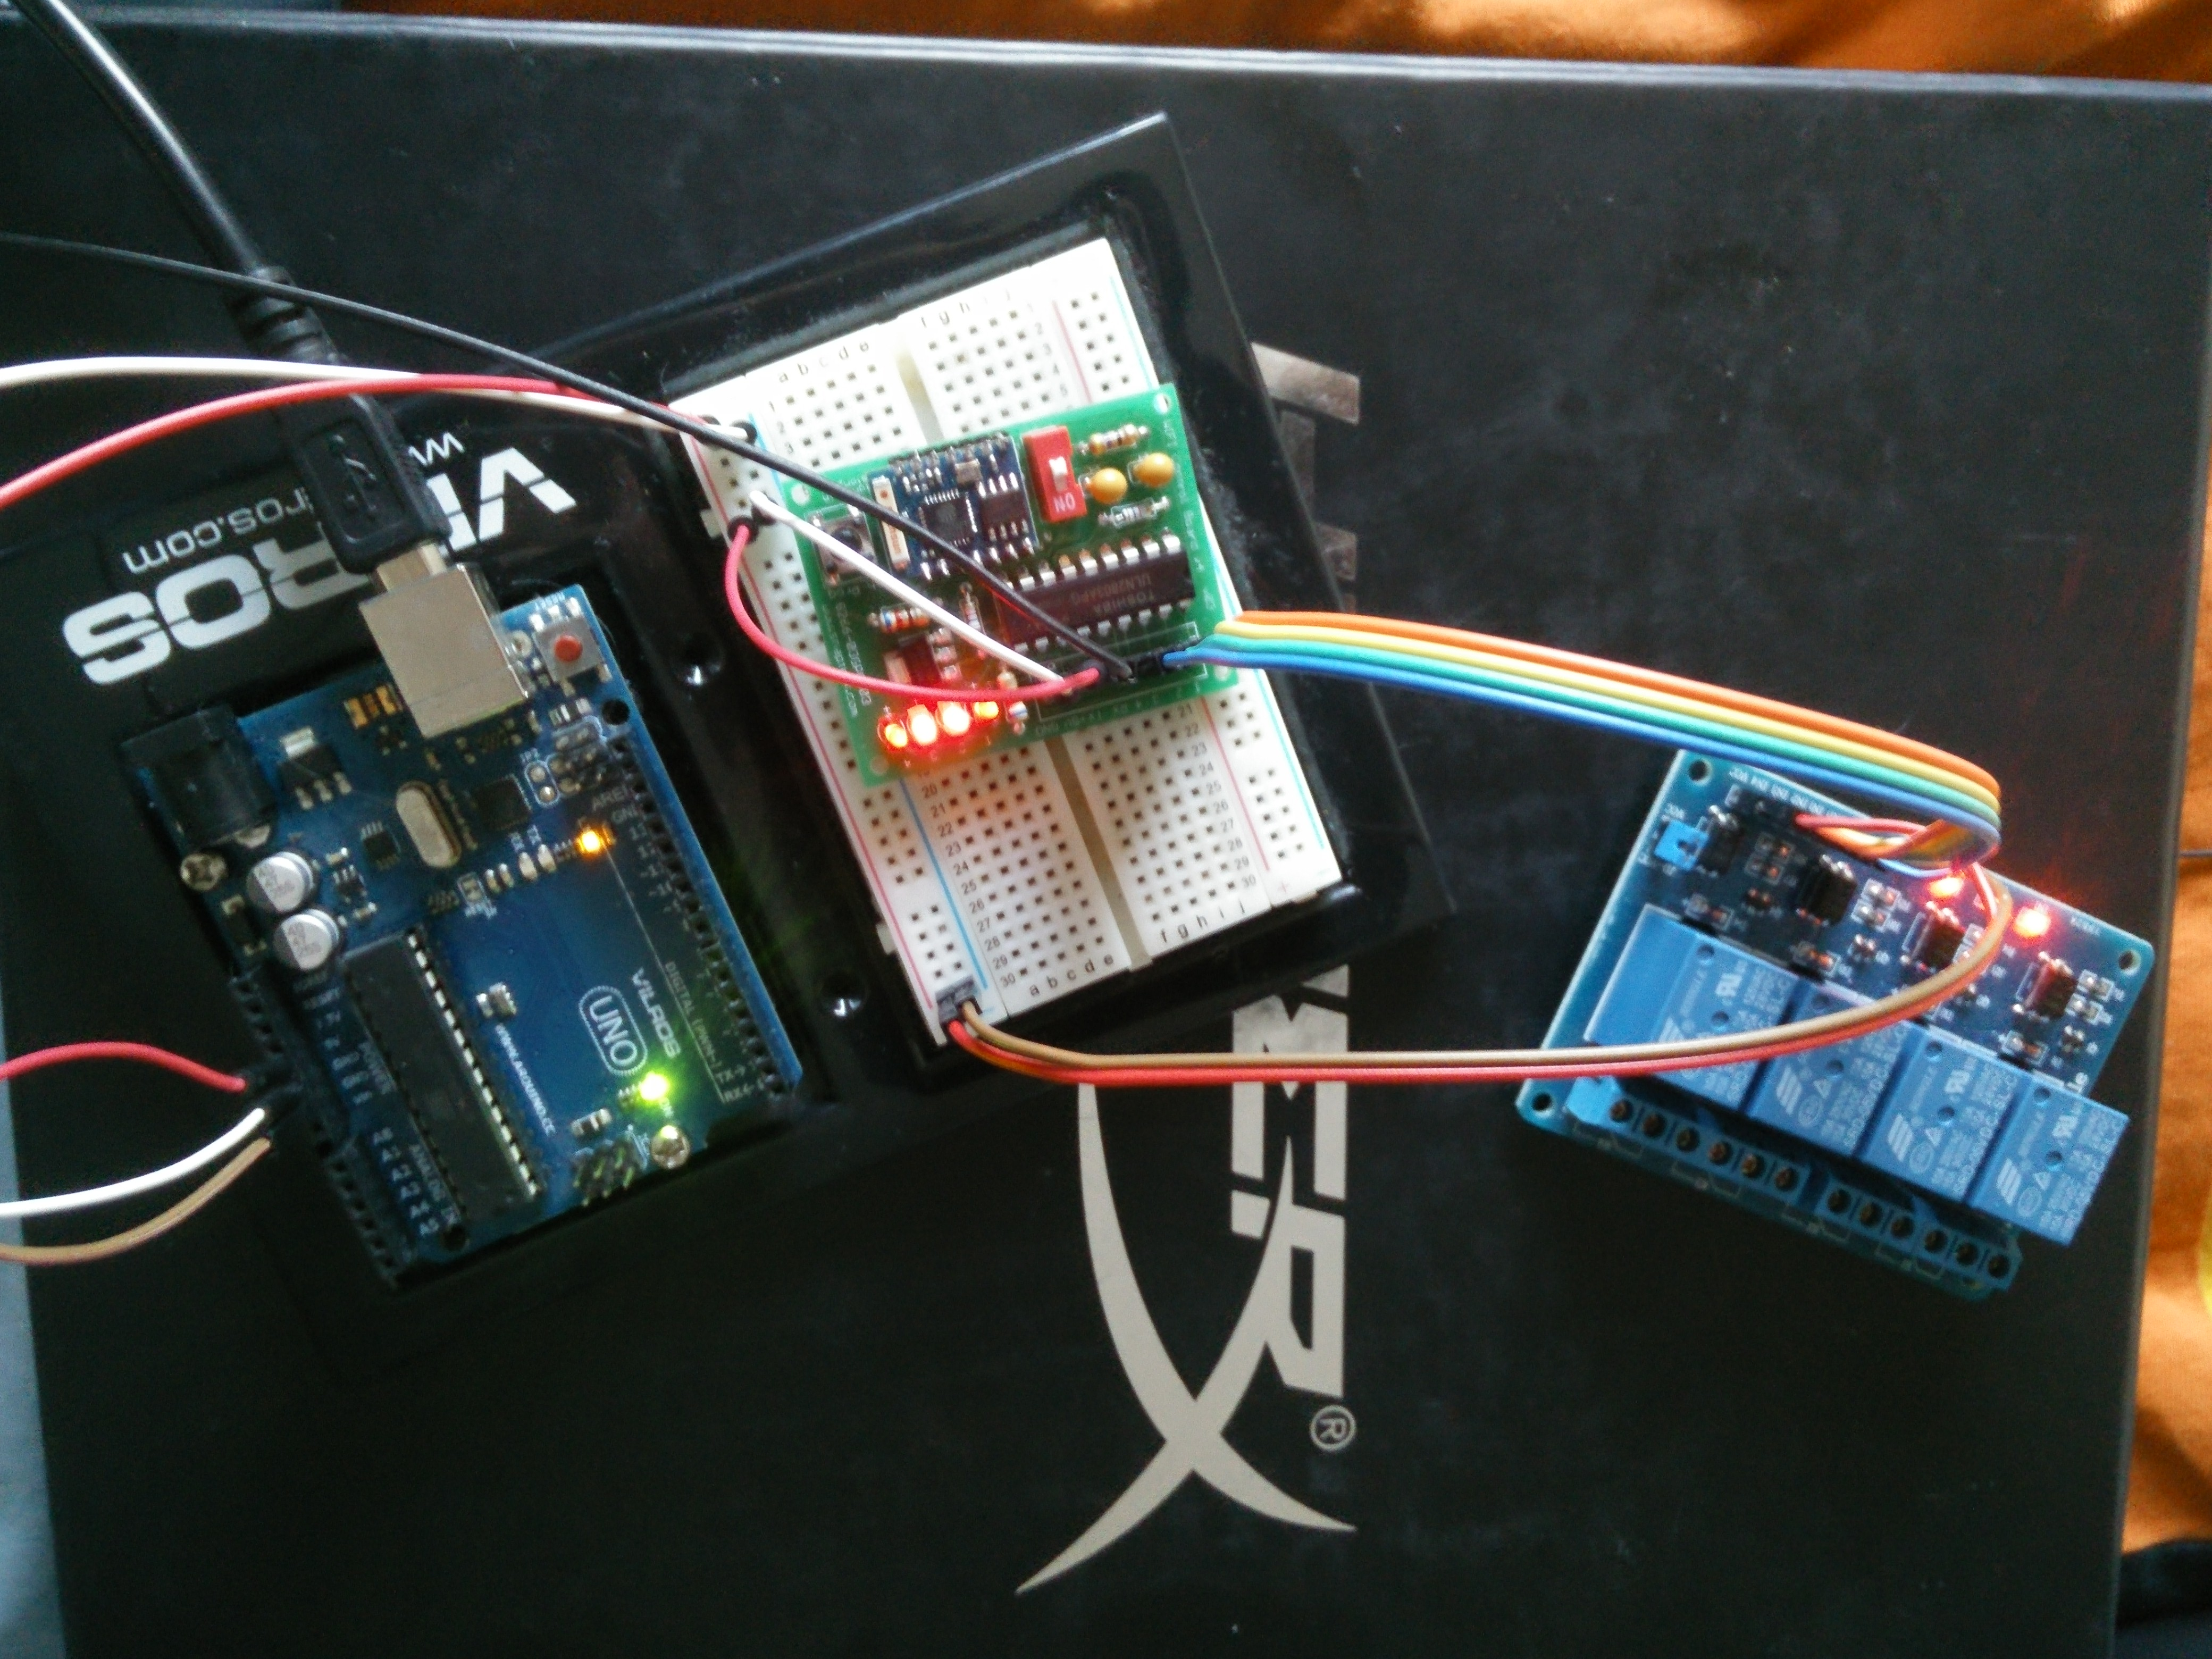
\includegraphics[scale=0.05]{circuit1}\\
Blog Date: 12-4-15

\subsection{Winter Update 1}
Over the break, our group refreshed our working knowledge of Flask, configured our new device for our Yocto build server and continued testing with the Raspberry Pi. We resumed work on the project and plan to meet during the weeks throughout the term to coordinate work, although most of our work will happen outside of our meetings. \\
Progress over break:
\begin{itemize}
\item Reviewed Python Flask to be better prepared to start working on it to build our web interface.
\item Configured the Raspbery Pi with software to run the web interface such as the ISC DHCP server and a basic DNS server.
\item Used Hostapd and wpa\_supplicant to have the Wifi adapter on the Pi broadcast an access point.
\end{itemize}
Week 1 work:
\begin{itemize}
\item Met to discuss web layout, decided on various Javascript libraries to run the application
\item Continued to develop software configuration for the Raspberry Pi and the corresponding Yocto image.
\end{itemize}
Problems:
\begin{itemize}
\item Some minor nonviolent disagreements on design for the front end of the application​ 
\end{itemize}
Plans for the coming week: 
\begin{itemize}
\item Continue development of front end application
\item Finish back-end scripts to send the commands to the ESP8266 module
\item Finish Python ISC-DHCP autodiscovery scripts
\end{itemize}
Blog Date: 1-8-16

\subsection{Winter Update 2}
Progress since last week:
\begin{itemize}
\item Changed requirements document to show that adjusting the brightness of lights is now a stretch goal. (requirements 1f, 2i, and 3m)
\item Created our first way to send the TCP command for turning on and off the lights.
\item Added database capability for the ESP devices.
\item Reformatted the layout of the website to be more compartmentalized and manageable.
\item Added python data structures for groups and lights
\end{itemize}
Problems:
\begin{itemize}
\item We realized that we would not be able to accomplish our goal of being able to adjust the brightness of the lights with the hardware we have available. We changed this goal to a stretch goal in the requirements document.
\end{itemize}
Plans for the coming week: 
\begin{itemize}
\item Continue development of front end application
\item Work more on connecting the website to the functions of the hardware
\end{itemize}
Blog Date: 1-15-16

\subsection{Winter Update 3}
Progress since last week:
\begin{itemize}
\item Added interface to add and view current connected ESP8266 devices, along with error handling.
\item Performed minor formatting and usability updates to the front page.
\item Created a basic Advanced page to accept dates/times for when to turn lights on/off and a basic query string that is able to live update via Javascript.
\end{itemize}
Problems:
\begin{itemize}
\item No notable problems this week.
\end{itemize}
Plans for the coming week: 
\begin{itemize}
\item Malcolm plans to work on making the front page of the site more usable by allowing the editing of names, the creation/deletion of groups, and the sending of reordering operations to the server from the web browser.
\item Sean plans to continue work on the Advanced page for creating rules for lights, including creating a proper query string and actually sending the updates back to the server.
\end{itemize}
Blog Date: 1-22-16

\subsection{Winter Update 4}
Progress since last week:
\begin{itemize}
\item Decided on a database layout for creating and displaying light groups on the front page of the site.
\item Continued to add support for the advanced page and improving the Javascript creating the custom queries.
\item Added login functionality and created a default user when the database is created. We'll actually apply the security to the pages when the project is near completion.
\end{itemize}
Problems:
\begin{itemize}
\item Minor disagreements on what to use for the group table structure, but resolved during Thursday's meeting.
\end{itemize}
Plans for the coming week: 
\begin{itemize}
\item Malcom will add the group display functionality to the front page, and will apply the \textit{jquery\_editable} functions to the group entries to allow easy editing of group attributes.
\item Sean will flesh out the logic generation subsystem as it interacts with the new light group management so that manual overrides are possible without disruption customized schedules.
\item Evan will finish the devices display and modification page by applying the \textit{jquery\_editable} package to it and will then work on the group layout with Malcom.
\end{itemize}
\subsection{Winter Update 5}
Progress since last week:
\begin{itemize}
\item Re-Wrote querybuilding on the server and started on the client's querybuilding.
\item Finalized the database schema and the flask sql-alchemy object relational model format.
\item Additional changes to the advanced page
\end{itemize}
Problems:
\begin{itemize}
\item No major problems this week.
\end{itemize}
Plans for the coming week: 
\begin{itemize}
\item We will work on and complete the Midterm Progress Report, as well as the accompanying video. 
\end{itemize}
Blog Date: 2-8-16

\subsection{Winter Update 6}
Progress since last week:
\begin{itemize}
\item Updated the formatting, fixed general bugs, and cleaned up the code for the website in both the advanced page and the main page
\item Finished the query builder for the advanced page
\item Rules now appear on the side when created
\item Finished both the progress report and the video to go along with it.
\end{itemize}
Problems:
\begin{itemize}
\item No major problems this week.
\end{itemize}
Plans for the coming week: 
\begin{itemize}
\item We will continue to work on achieving beta-level functionality for all parts of the project
\end{itemize}
Blog Date: 2-12-16

\subsection{Winter Update 7}
Progress since last week:
\begin{itemize}
\item Implemented sorting on the Flask app's front page for groups
\item Added JS for deleting groups and adding of new groups
\item Continued logical development for the advanced page and custom user queries
\item Fixed some minor styling bugs with custom CSS
\end{itemize}
Problems:
\begin{itemize}
\item No major problems this week.
\end{itemize}
Plans for the coming week: 
\begin{itemize}
\item Continue working on the advanced user queries
\item Implement group change interaction with the database on the front page
\end{itemize}
Blog Date: 2-19-16

\subsection{Winter Update 8}
Progress since last week:
\begin{itemize}
\item Reorganized advanced page layout for usability according to feedback from user study.
\item Removed ability to apply multiple rules to each light/group to improve usability, since users found the concept of multiple rules per light/group confusing.  No functionality is lost, however, since parent group rules can still be applied, and custom queries can be created that achieve the same result as multiple rules.
\begin{itemize}
\item Since each light/group only has one rule now, the rules table was removed from the database and a rule column was added to the light and group tables.
\end{itemize}
\item Advanced page now sends rule changes to the server via AJAX, updating the database immediately whenever a change is made.  This negates the need for the user to hit a "save changes" button or the like, which users responded poorly to in the user study.
\item Fixed bug with deleting groups that have nested group children on the main page.
\item Fixed additional minor styling bugs, such as with the light/group name editing box on the main page appearing on a new row.
\end{itemize}
Problems:
\begin{itemize}
\item No major problems this week.
\end{itemize}
Plans for the coming week: 
\begin{itemize}
\item Implement job for re-evaluating rules on startup and periodically, including calculating proper sunset/sunrise times, and then sending updates to each light.
\item Make further style/usability tweaks to site, including front page and advanced page, such as making buttons bigger, adding help text, fixing alignment of elements, etc.
\item Create settings page
\begin{itemize}
\item Currently, only planned setting is for geographical location for calculating accurate sunset/sunrise times.
\end{itemize}
\item Intregation testing
\begin{itemize}
\item Starting from an empty database, add a new client device and toggle the lights from the main web UI and through rules.
\item Test the use of the website on the Pi's touchscreen.
\end{itemize}
\end{itemize}
Blog Date: 2-26-16

\subsection{Winter Update 9}
Progress since last week:
\begin{itemize}
\item As we near the end of our project, we have started using Github's issue tracker for all bugs and yet-to-be-implemented features:
\begin{itemize}
\item https://github.com/rettigs/cs-senior-capstone/issues
\end{itemize}
\item Essentially finished beta version of project, completing all high priority issues.
\item The main portion of the project that was finished was the advanced page and rule system; the advanced page has been reformatted to make it easier to use, and the rule system was overhauled to use custom datetime wrapper objects to elegantly handle early/late toggle times and randomized toggle times.
\begin{itemize}
\item We also implemented sunset/sunrise time calculation using the Astral Python module and adding a settings page that allows the user to select their geographic location.
\item Furthermore, the scheduler that actually runs the rules periodically has been implemented, using the Schedule Python module.
\end{itemize}
\item We have performed integration testing involving using all of the main features of the project (e.g. toggling lights manually, using rules, using groups, etc.) on the provided hardware and all of the functionality is there, save for a few minor bugs.
\item We have updated our poster to reflect the current status of the project.
\item We have created a slideshow presentation for use as an outline for our final video presentation.
\end{itemize}
Problems:
\begin{itemize}
\item It was fairly minor, but originally, we had issues with the rule system ignoring manual overrides; whenever a user manually toggled a light, the rule system would overwrite it the next time it ran.
\begin{itemize}
\item This was solved by making sure that the overridden state of a light was stored in the database and making rules check if a light is overridden before updating it.
\end{itemize}
\end{itemize}
Plans for the coming week: 
\begin{itemize}
\item Resolve all medium-priority issues.  Fixing low-priority issues will be our goal next term, as they are mostly minor usability and maintainability improvements that are not necessary for a beta release. 
\item Finish poster and slideshow
\item Finish video and progress report
\end{itemize}
Blog Date: 3-8-16

\subsection{Winter Update 10}
Progress since last week:
\begin{itemize}
\item Continued work on isses for the project, including adding new ones since week 9 and resolving outstanding ones
\begin{itemize}
\item Total issues currently open: 9 (all low-priority)
\item 19 issues closed: 11 medium, 3 high priority
\end{itemize}
\item The full unit test with the screen, mobile device, and relay connected to LEDs was conducted. The tests revealed bugs that were caught and fixed.
\begin{itemize}
\item For instance, we found out that we needed to reverse the logic for generating the TCP commands to make the relay function properly.
\end{itemize}
\item We created our presentation video for the physical device and began shooting video for our powerpoint presentation
\item We finalized our poster after review and submitted the final revision
\end{itemize}
Problems:
\begin{itemize}
\item The lights on the relay were out of sync, we fixed this by logically flipping the TCP command sent to the ESP module
\item The override function did not match the requirements document, so Sean revised the override logic to match the requirement.
\end{itemize}
Plans for the coming week: 
\begin{itemize}
\item Finish video and progress report
\end{itemize}
Blog Date: 3-11-16

\subsection{Spring Update 1}
At this point, our project is at a completed stage, but we have identified a few bugs and usability issues that we will spend this term working on.\\
Progress at start:
\begin{itemize}
\item We met to discuss adding new issues to work on this term as enhancements to the final product. Our first priority is to complete two new medium-level issues before the Expo:
\begin{itemize}
\item Create a JS poller so that the lights update on all open pages when the rules or a user changes them.
\item Change the default names for lights so that they're user-friendly.
\end{itemize}
\item Evan has been using the system at home to run his own lights as part of a long term test. The test began on 3/31/16 and will be updated as we get closer to expo.
\item We added the Yocto layer for the build and the site itself to the Github repo, and will be updating the Readme to add the proper Yocto version and machine type.
\end{itemize}
Problems:
\begin{itemize}
\item We had no major issues, and since the finished product (minus usability changes and bug fixes) has been demonstrated and is in long-term testing, we don't expect many production issues at this point.
\end{itemize}
Plans for the coming week: 
\begin{itemize}
\item Resolve all medium-priority issues.
\end{itemize}
Blog Date: 4-4-16

\subsection{Spring Update 2}
Progress this week:
\begin{itemize}
\item We met with our client, Victor, to demonstrate the state of our project and receive feedback.  Some of the suggestions from the meeting include:
\begin{itemize}
\item Make sure to account for daylight savings time.
\item Make rules run more often than every 60 seconds, especially for demos.
\item Make rules run immediately when rules are changed.
\item Include a way to simulate time running faster, especially for demos.  This could potentially allow a whole daily cycle to be simulated in just seconds, showing off the rule system in a timely fashion.
\item Improve our physical demo setup; our current setup involves a breadboard, an extra Arduino for power, and a lot of stray wires; our new plan is to have a small model house made from PCB with the LEDs soldered in and hooked up directly to a 120V to 5V converter.  We also plan to have 2 ESP/relay units for the final demo, which Victor has ordered for us.
\end{itemize}
\item We also started work on some of our highest-priority issues, particularly the client-side polling to automatically update light statuses without refreshing, and checks to prevent light statuses from changing if a toggle action failed (such as if the power strip was unplugged or there was wireless interference).
\end{itemize}
Problems:
\begin{itemize}
\item One problem we had was that during the demo with our client, the rules did not seem to trigger when they should have.  However, we later realized that we had been manually toggling the lights immediately beforehand, which overrode the rules; the behavior was actually intended.  We need to remember this in future demos.  The faster time simulation could help with this since even if we override the lights, the override period will end much more quickly.
\end{itemize}
Plans for the coming week: 
\begin{itemize}
\item Finish and submit final version of expo poster
\item Complete high priority issues
\item Prepare model for expo
\end{itemize}
Blog Date: 4-13-16

\subsection{Spring Update 3}
Progress this week:
\begin{itemize}
\item Added a function to the test branch for the int\_bool conversion to make the code involved with clicking the group buttons cleaner.
\item Removed the duplicate add\_device function, and cleaned up the original by making better default names.
\item Started building a rough model house to use at expo using junk pcb.
\item Started work on the poller which checks the status of the lights and updates them for the client if they have changed.
\end{itemize}
Problems:
\begin{itemize}
\item Our int\_bool conversion branch is still not toggling all of the lights in a group correctly when one of the group control buttons is pressed
\end{itemize}
Plans for the coming week: 
\begin{itemize}
\item Debug and fix the problem with the int\_bool conversion branch
\item Continue working on and possibly finish the pcb model house
\item Polish up the poster so that it can be submitted at the end of next week
\item Complete high priority issues
\end{itemize}
Blog Date: 4-15-16

\subsection{Spring Update 4}
Progress this week:
\begin{itemize}
\item Polished the poster and submitted it to the TA for review
\item Constructed the first prototype for the house model for use at expo (pictured below)
\item Completed changing entry in database for light status from integers to booleans
\item Completed the poller to update the switch status across windows.
\end{itemize}
Problems:
\begin{itemize}
\item No major issues encountered this week
\end{itemize}
Plans for the coming week: 
\begin{itemize}
\item Complete all medium-level issues
\item Complete the next prototype for the house model for expo
\end{itemize}
Blog Date: 4-24-16
